\documentclass{IEEEtran}
\usepackage{mathtools}
\usepackage{graphicx}
\usepackage{amssymb}
\usepackage{amsmath}
\usepackage{pythonhighlight}
\usepackage[utf8]{inputenc}
\usepackage{fancyhdr}
\usepackage{pythonhighlight}
\usepackage{changepage}
\usepackage{slashbox}
\usepackage{floatrow}
\usepackage{listings}
\usepackage{derivative}
\usepackage[hidelinks]{hyperref}
\usepackage{fontawesome}
\usepackage{caption}
\usepackage{subcaption}
\usepackage[sorting=none,style=ieee]{biblatex}
\usepackage{cleveref}
\usepackage{algorithm}
\usepackage{algpseudocode}

\addbibresource{report.bib}
\title{Hodgkin and Huxley Cell Membrane Model Simulation}
\author{Kutay Ugurlu}

\begin{document}
\maketitle
\begin{abstract}
    The electrical behaviours of specific kind of organs and structures in human body provide crucial information about the workings of physiological level structures and mechanisms of certain diseases. For diagnosis regarding such structures, many imaging methods have been developed exploiting these behaviors. To do so, a good understanding of the electrical cell behavior is required. This report provides a theoretical background for the action potential behavior, using Hodgkin-Huxley's explanation and explains the methodology to create a simulation software that illustrates the generation and propagation of the action potentials. 
\end{abstract}
\section{Intro}
Hodgkin and Huxley \cite{hodgkin1952quantitative} published a series of five paper in 1952 to explain the generation mechanism of the action potential by introducing their experimental setup and the method. The first paper focused on explaining how the nueron cells work. The second paper investigated the relationship between sodium ion concentration and the membrane voltage, also mentioning the action potential behavior. The third paper examined the effect of sudden conductance changes in the generation of the action potential. It was the fourth paper where Hodgkin and Huxley first explained the sodium inactivation phenomenon. In the last paper, the authors compiled their experimental results and came up with a formulation that explains the action potential generation process. 

\subsection{Voltage Clamp Experiment}

\begin{figure}[h]
\centering
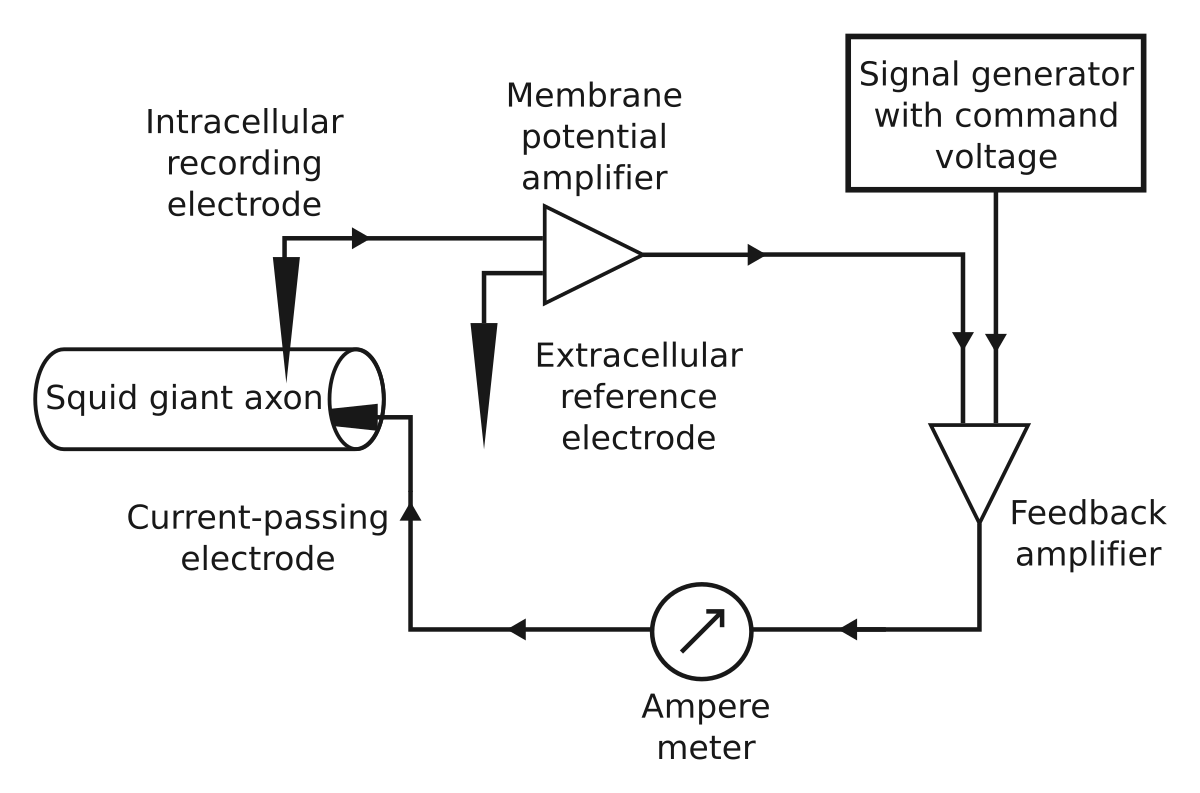
\includegraphics[width=\textwidth]{VCE.png}
\caption{Voltage Clamp Experiment Setup}\label{fig:vce}
\end{figure}

Voltage clamp is an experimental setup to measure the ionic currents that produce the electrical behavior of the excitable cells. It utilizes an iterative feedback mechanism, and the corresponding circuit, to achieve the desired or set voltage level of the membrane potential. Keeping the equivalent circuit model \Cref{fig:eqcct} and the equations governing the node voltage relations in this circuit, the researchers clamped the voltage at the Nernst potential and observed the transient and steady-state behavior of the resultant ionic currents. The measurement provided by these experiments paved the way to discovering the analytical relationship between cell membrane voltage and ionic conductances via curve fitting. 

\section{Theory}

\subsection{Mathematical Model}
\subsubsection*{Conductance}
The instantaneous conductances of different ion channels are calculated using the following relations:

\begin{align}
    g_{Na} &= m^3h \overline{g_{Na}} \\
    g_{K} &= n^4 \overline{g_K} \\
    g_{L} &= \overline{g_{L}}
\end{align}

The parameters that control the change of conductances in terms of deviation from membrane voltage, \textit{i.e.} negative depolarization $V_{rest} - V_m$, are also expressed in first order linear differential equations of time as follows:

\begin{align}
    \pdv{n}{t} &= \alpha_n(V_m)(1-n) - \beta_n(V_m)n \label{eqn:pdv1}\\
    \pdv{m}{t} &= \alpha_m(V_m)(1-n) - \beta_m(V_m)n \label{eqn:pdv2}\\
    \pdv{h}{t} &= \alpha_h(V_m)(1-n) - \beta_h(V_m)n \label{eqn:pdv3}\\
\end{align}

where $V_m$ is the deviation. \\

\subsubsection*{Activation and Inactivation Parameters}
The activation and inactivation parameters given in \Cref{eqn:pdv1,eqn:pdv2,eqn:pdv3} are formulated via curve fitting in Hodgkin and Huxley experiments. The resultans formulation are provided in \Cref{eqn:a1,eqn:a2,eqn:a3,eqn:b1,eqn:b2,eqn:b3}.

\begin{align}
    \alpha_n(V_m) &= \frac{0.01(10-V_m)}{e^{(1-0.1V)}-1} \label{eqn:a1}\\
    \alpha_m(V_m) &= \frac{0.01(25-V_m)}{e^{(2.5-0.1V)}-1} \label{eqn:a2}\\
    \alpha_h(V_m) &= 0.07e^{(\frac{-V}{20})} \label{eqn:a3}\\
    \beta_n(V_m) &= 0.125e^{(\frac{-V}{80})} \label{eqn:b1}\\
    \beta_m(V_m) &= 4e^{(\frac{-V}{18})} \label{eqn:b2}\\
    \beta_h(V_m) &= \frac{1}{e^{(3-0.1V)}-1} \label{eqn:b3}
\end{align}
\\
\\

\subsubsection*{Equivalent Circuit Model}
\begin{figure}[h]
\centering
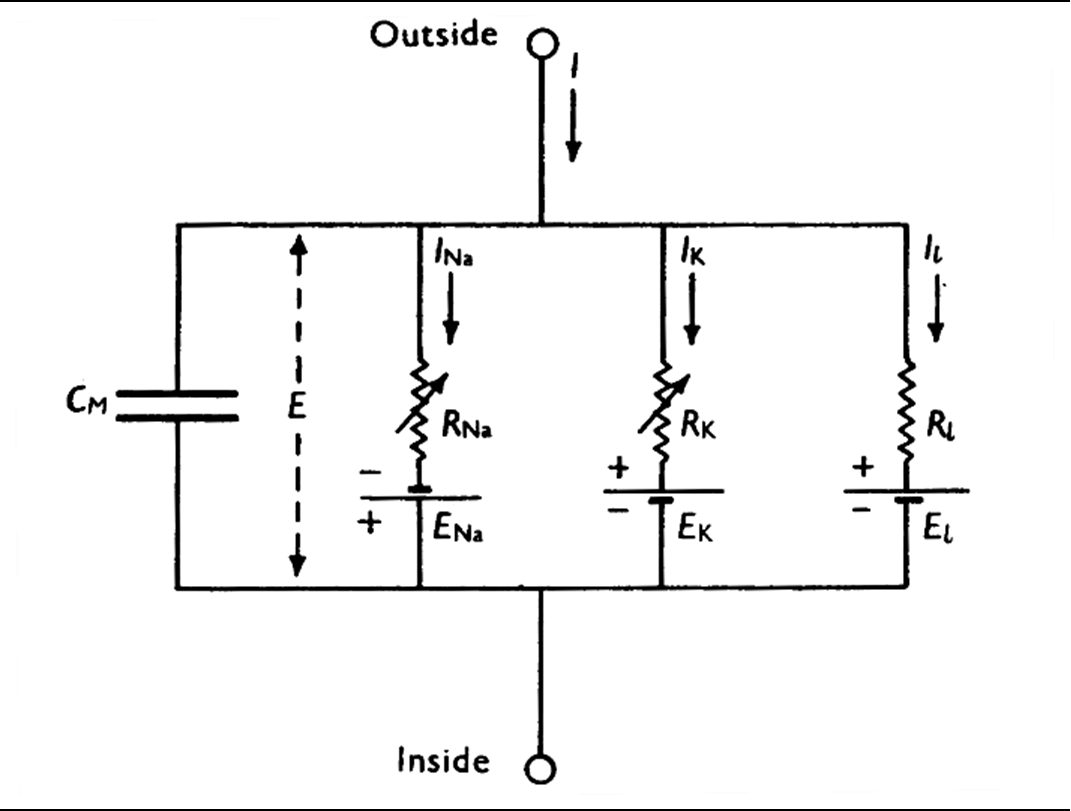
\includegraphics[width=0.8\textwidth]{EQCCT.png}
\caption{Equivalent Circuit of Hodgkin and Huxley membrane model}\label{fig:eqcct}
\end{figure}

Employing the node relations on the equivalent circuit, one can derive the relations given in \Cref{eqn:node1,eqn:node2,eqn:node3,eqn:kirch1,eqn:kirch2} for any time, hence any value of negative depolarization.

\begin{align}
    I_{Na} &= g_{Na}(V_{membrane} - E_{Na}) \label{eqn:node1}\\
    I_{K} &= g_{K}(V_{membrane} - E_{K}) \label{eqn:node2}\\
    I_{Cl} &= g_{L}(V_{membrane} - E_{Cl}) \label{eqn:node3}\\
    I_{ionic} &= I_{Na} + I_{K} + I_{Cl} \label{eqn:kirch1}\\
    I_{Capacitive} &= I_{total} - I_{ionic} \label{eqn:kirch2}
\end{align}

where $I_{total}$ is the stimulation current applied to the cell. 

\subsection{Method}
\subsubsection{Generation}

For the generation part of the algorithm, 

\begin{algorithm}
    \caption{An algorithm with caption}\label{alg:cap}
    \begin{algorithmic}
    \Require $n \geq 0$
    \Ensure $y = x^n$
    \State $y \gets 1$
    \State $X \gets x$
    \State $N \gets n$
    \While{$N \neq 0$}
    \If{$N$ is even}
        \State $X \gets X \times X$
        \State $N \gets \frac{N}{2}$  \Comment{This is a comment}
    \ElsIf{$N$ is odd}
        \State $y \gets y \times X$
        \State $N \gets N - 1$
    \EndIf
    \EndWhile
    \end{algorithmic}
\end{algorithm}


\clearpage
\printbibliography{}
\end{document}

